\chapter[Operating System State Pausing and Virtual Storage Device \\ Co-Simulation]{Operating System State Pausing and Virtual Storage Device Co-Simulation}
\label{ch:3}

This dissertation proposes a novel OS state pausing approach to storage device emulation that allows simulated virtual storage device to be co-simulated with OS and application programs running on real computer hardware. The key idea of the proposed approach is to modify the OS in a way that its execution state can be paused and resumed, even while the OS is being run on unmodified real computer hardware. This means that the flow of time that is observed by the OS and application programs can be controlled discretely and is no longer hardwired to the real-world time. By properly controlling the execution state of the OS and synchronizes it with the simulation progression of the virtual storage device, the simulated virtual storage device can be made to co-simulate with the real computer system that runs the modified OS in the discrete-time domain. The resulting co-simulation environment can be used for conducting studies on the simulated virtual storage device and the corresponding storage subsystem in realistic full-system contexts.

One way to understand the proposed co-simulation approach is that the real physical hardware is used as part of the full-system simulation model. In the complete machine simulation approach, a detailed model of the target system's hardware needs to be constructed and used for running the software programs. The hardware model needs to be detailed enough so that it can execute the real OS and application programs. It's performance characteristics also needs to be precise enough so that the performance evaluation results predicted using the complete machine model will be representative of the real world results. In other words, only achieving behavioral correctness with the simulated hardware model is not enough for conducting full-system performance evaluations.

With the proposed co-simulation approach, the OS is running on the real computer hardware. This means that the detailed characteristics of the CPU and memory subsystems will be taken into account when the co-simulation model is used for generating workloads towards the virtual storage device or for conducting full-system performance evaluations. Furthermore, utilizing the real hardware to run the software programs will be faster then running them on virtually simulated hardware models.

The key concept of the proposed co-simulation methodology is to control the execution state of the OS and make the OS to observe a virtual system time that is not hardwired to the real world clock. In the work of Gupta~\cite{Gupta:2006}, they proposed a technique called \textit{time dilation} to make the OS to observe a passage of time that is a constant time slower than the real-time clock. From the OS’s perspective, the physical resources in the external world will appear to be faster than their original speeds. For example, if the passage of time observed by the OS is slowed down by 10 times, then data arriving from a network interface at a physical rate of 1Gbps would appear to the OS as arriving at 10Gbps. They have demonstrated that \textit{time dilation} is an effective method for emulating network interfaces of different speeds to the OS for end-to-end system behavior experimentations. 

Although the proposed storage device emulator also makes the OS to observe a passage of system time that is different than the real-time clock, the goal and mechanisms are different from those of \textit{time dilation}:

\begin{itemize}
	\item  In \textit{time dilation}, the passage of system time is only slowed down by a constant factor but will never be stopped. In other words, the OS is always executing continuously. In contrast, in our proposed OS state pausing approach, the execution of the OS will be paused as necessary whenever the storage device emulator is busy processing the I/O requests. The goal of \textit{time dilation} is to trick the OS into believing that the external resources are faster than what they actually are. On the other hand, the goal of OS state pausing is to temporarily freeze the execution of the OS so that the storage device emulator can spend unlimited amount of time on processing the I/O requests.
	
	\item The slowing down of the passage of time in \textit{time dilation} is achieved by reducing the frequency that the timer interrupts are delivered to the OS and also by appropriately scaling down the hardware time counter that is used by the OS. For example, to slow down the passage of time observed by the OS by 10 times, the timer interrupt frequency is reduced by 10 times and the hardware time counter is also scaled down by 10 times. In comparison, pausing the state of the OS requires stopping the hardware time counter and preventing the CPU from doing any work for the OS.
	
	\item The design of the proposed storage device emulator can be extended with \textit{time dilation}. In the proposed emulator design, the OS can either be in the paused state or in the running state. When in the running state, it is possible to apply \textit{time dilation} so that the OS will observe that it is running on a CPU which is faster than the CPU of the target system. However, in order to keep our focus, we do not apply \textit{time dilation} to the proposed storage device emulator in this article.
\end{itemize}

The concept of OS state pausing is discussed in section~\ref{sec:controlling-OS-state}. Section~\ref{sec:OS-state-pausing-and-storage-device-emulation} gives an overview of how OS state pausing is used to allow virtual storage device to be co-simulated with real computer system running real OS and application programs. Section~\ref{sec:synchronization-granularity} discusses the synchronization considerations between the state of the simulated virtual storage device and the state of the OS. The idea of time-skipping the CPU idle loop, which can be used to accelerate the co-simulation process, is discussed in section~\ref{sec:time-skipping}.

\section{Controlling the Operating System State}
\label{sec:controlling-OS-state}

The key of being able to co-simulate the OS running on unmodified real computer hardware with simulated virtual storage device in the discrete-time domain is the ability to control the state progression of the OS. That is, we need to be able to pause and resume the running state of the OS on unmodified computer hardware.

\begin{figure}[htpb]
	\centering
	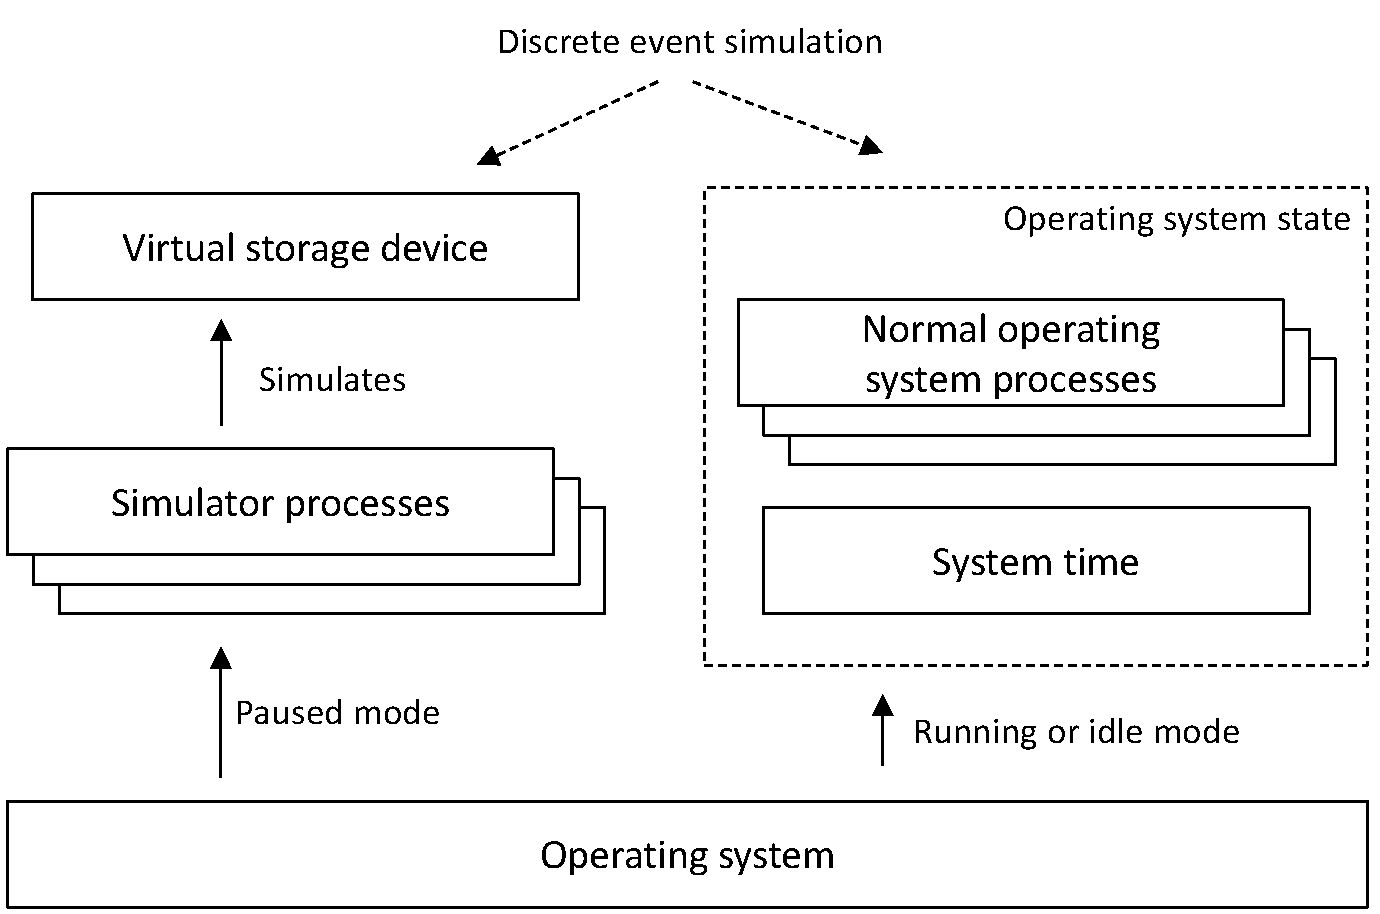
\includegraphics[width=0.8\textwidth]{figures/ch3-OS-state.pdf}
	\caption{\label{fig:ch3-OS-state}OS state pausing and discrete event simulation.}
\end{figure}

As illustrated in Figure~\ref{fig:ch3-OS-state}, the state of an OS can be viewed as composed of the combined state of all the normal processes running in the OS and the values in the clock counter and the hardware timers referenced by the OS. By freezing the execution of all the normal processes in the OS and stopping the clock counter and the hardware timers, the state of the OS is paused. The ``normal'' operating system processes are referring to the processes that are part of the original unmodified OS. On the other hand, the ``simulator'' processes are processes that do not exist in the original OS and are responsible for performing tasks such as storage device simulation while the OS is in the paused state.

By properly control the state progression of the OS, the OS can be co-simulated with the virtual storage device to form a full-system simulation environment. The OS can be put into one of the three following modes during the co-simulation process:

\begin{itemize}
	\item \textbf{Pause mode} --- In this mode, the progression of the OS state is frozen. All of the normal processes are prevented from being run on the CPU and the clock counter and hardware timers are paused. When in the paused mode, the system time that is perceived by the OS is no longer advancing and the CPUs are not performing any useful work for the OS. The simulator processes are executed only when the OS is in the paused mode, and therefore the execution of the simulator processes will not affect the original behavior of the OS.
	
	\item \textbf{Running mode} --- In the running mode, the OS state is advancing continuously with regarding to the real-world clock. That is, for every second that the OS is put into the running mode, the OS state is advanced one second into the future. In the running mode, the normal processes are selected to run on the CPU according to the task scheduling policy of the OS. All of the clock counter and hardware timers that the OS reference are operating normally.

	\item \textbf{Idle mode} --- The idle mode is a special case of the running mode. The OS is said to be in the idle mode when the OS is in the running mode but that the CPU is executing the CPU idle process. In this mode, all the normal processes excluding the CPU idle process will remain in the same states. Observe that while the OS is in the idle mode, the only OS state that is changing is the system time. Therefore, it is possible to fast-forward the system time to a future time point so that the simulation process does not spend unnecessary time waiting in the idle mode. The ``time-skipping'' feature what will be further discussed in section~\ref{sec:time-skipping}.
\end{itemize}

\section{Storage Device Emulation and Discrete Event Simulation}
\label{sec:OS-state-pausing-and-storage-device-emulation}

The proposed co-simulation methodology is based on the concept of storage device emulation and discrete event simulation. In the timing-accurate storage device emulation methodology of Griffin et al.~\cite{Griffin:2002}, a virtual storage device with timing behaviors matching the target device is plugged into the OS. The virtual storage device along with other modules in the OS forms the storage subsystem. The entire system operates in the real-time domain. Real applications running on the OS can be used for generating benchmark workloads towards the simulated storage device.

In the proposed methodology, a virtual storage device is emulated to the OS at the block device driver level and its simulation state is synchronized with the state of the OS. Whenever there is an I/O request received by the emulated storage device, the OS is put into the paused mode while the storage device emulator is busy preparing the I/O response. The OS is put back to the running mode when the timing for the I/O response is determined. A timer event that references the virtual system time is used to submit the I/O response to the OS when the corresponding response time has arrived. Because of the pausing made to the OS state, the OS and the virtual storage device can be viewed as being co-simulated together in the discrete-time domain.

In summary, the key difference between timing-accurate storage device emulation and the proposed co-simulation methodology is the time domain that the whole system operates in. In timing-accurate storage device emulation, the simulation time of the virtual storage device emulator is synchronized with the real-word clock. Both the OS and the virtual storage device are operating in the real-time domain. That is, the state of the entire system progresses according to the real-world clock. In contrast, in the proposed co-simulation approach, the OS and the virtual storage device are simulated together in the discrete-time domain.

The key advantages of the proposed OS state pausing full-system co-simulation approach compared to the timing-accurate storage device emulation approach are summarized as follows.

\begin{itemize}
	\item The OS state can be paused. This means that the storage device simulation module can take as long as it needs for preparing the I/O responses without affecting the performance of the storage device as perceived by the OS. In comparison, in the timing-accurate storage device emulation approach, each individual I/O request must be responded back to the OS at exactly the desired service time of the disk model. Otherwise, the emulated storage device will have a performance characteristic that is different from the intended target. In other words, the storage device simulation module must be able to prepare the I/O responses in real-time.

	\item It is possible for the proposed full-system co-simulation environment to be simulated at a speed that is faster than real-time. In the timing-accurate storage device emulation approach, the OS is operating in the real-time domain using the real-world clock as its system time. This means that the entire evaluation process is constrained to proceed at the real-time speed. On the other hand, with the proposed co-simulation approach, the OS state can be fast-forwarded to speedup the simulation process whenever the CPU is in the idle loop due to waiting for the I/O response from the emulated storage device.
\end{itemize}

\section{Synchronization Granularity}
\label{sec:synchronization-granularity}

In discrete event simulation, a simulation model of the target system is constructed and its state is changed by a chronological sequence of discrete events. The simulation model of the proposed full-system co-simulation environment contains two parts:
\begin{enumerate*}[label=(\roman*)]
	\item the OS running on the real machine hardware, and
	\item the storage device simulator.
\end{enumerate*}
During simulation, the two parts of the simulation model need be advanced in a synchronized fashion so the overall system behavior is correct. That is, the state progression of the OS needs to match with the state progression of the simulated storage device. For example, if the OS submits an I/O request to the simulated storage device at time $t$ and it takes the
device $\Delta t$ amount of time to complete the I/O request, then it is important that when the I/O response is replied back to the OS, the system time of the OS is at $t + \Delta t$.


In the conventional full machine simulation approach, the synchronization between the OS and the storage device is achieved automatically by running the OS on the simulated machine hardware model. Due to the storage device is part of the machine hardware model, the OS state will automatically be synchronized with the state of the storage device. Depending on the design, the state advancement of the entire simulation model can be progressing at different granularities. For example, it could be at the per clock cycle or the per CPU instruction levels. Although extremely accurate, this kind of fine-grained synchronization between the OS and the simulated device is not necessary for evaluating storage subsystem designs.

\begin{figure}[htpb]
	\centering
	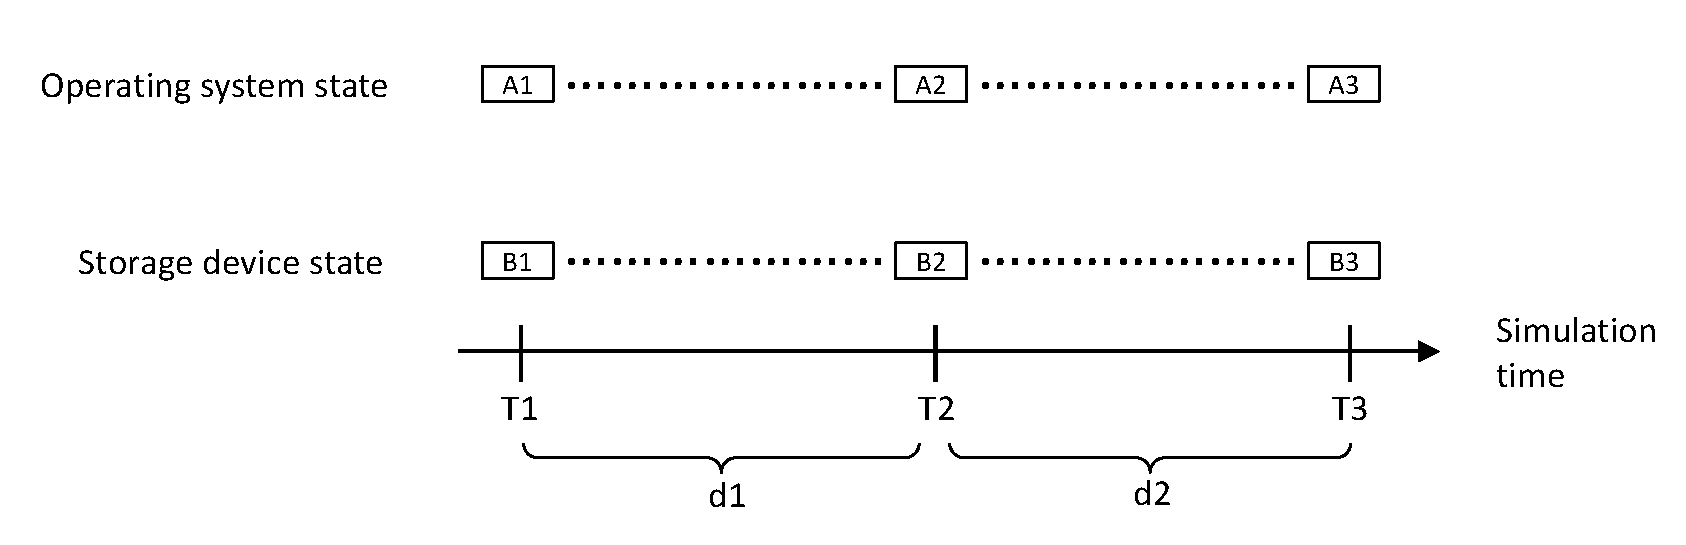
\includegraphics[width=0.95\textwidth]{figures/ch3-sychronization-granularity.pdf}
	\caption[Synchronization between the OS and the simulated storage device.]{\label{fig:ch3-sychronization-granularity}For evaluating storage subsystem designs, the states of the OS and the simulated storage device only need to be synchronized at the I/O event level.}
\end{figure}

The observation is that for evaluating storage subsystem designs, synchronizing the state of the OS and the state of the simulated storage device at the I/O event level is sufficient for capturing the overall system behavior. Figure~\ref{fig:ch3-sychronization-granularity} is used to explain this concept. Assuming that a simulation model that contains an OS and a storage device is being simulated, when the simulation begins at time point T1, both the OS and the storage device are in their initial states A1 and B1, respectively. After d1 amount of time, at simulation time point T2, the OS submits an I/O request to the storage device, and the storage device simulator determines that it requires d2 amount of time to process the I/O request. After d2 amount of time, the I/O response is replied back to the OS at simulation time point T3. Observe that for the purpose of evaluating storage subsystem designs, synchronizing the simulation states of the OS and the storage device at time point T1, T2, and T3 is sufficient for capturing the overall system behavior. That is, the co-simulation environment only needs to make sure that when the OS is at state A2, the storage device is at state B2; similarly, when the OS is at state A3, the storage device is at state B3. The intermediate states between A1 and A2, or A2 and A3, do not need to be explicitly synchronized with the intermediate states between B1 and B2, or B2 and B3. In other words, the co-simulation environment only needs to make sure that the entire simulation model is in a synchronized state when the OS is interacting with the simulated storage device. The intermediate states that the OS goes through internally do not need to be synchronized explicitly with the internal intermediate states of the simulated storage device.

\section{Time-Skipping --- Fast Forwarding the CPU Idle Loop}
\label{sec:time-skipping}

When the OS is in the idle mode, the CPU is simply waiting in an indefinite idle loop and not doing any useful work. That is, the OS is simply waiting for the system time to pass by so that some process will become runnable again. To speedup the simulation process, it is possible to time-skip the CPU idle loop by fast-forwarding the system time to a future time point. As soon as the OS enters the idle mode, the simulation kernel determines the future system time point at which there will be a process to become runnable again. The system time is then fast-forwarded to that future time point and the OS can get out of the idle mode immediately. This operation is called ``time-skipping'' the CPU idle loop.

Notice that the OS state will be the same when it finally leaves the idle mode either with or without applying the time-skipping feature to skip the CPU idle loop. This is because the only OS state parameter that will be changed while the OS is in the idle mode is the system time. The states of all the other processes in the OS will remain unchanged. Therefore, to the OS state, fast-forwarding the system time to a future time point at which some process will become runnable again is equivalent for the CPU to actually wait in the CPU idle loop and waits for the corresponding amount of time to pass by.

When the storage subsystem is being benchmarked, there will always be at least one process in the OS waiting in the sleep state. In general, the benchmark application could go into the sleep state because it is waiting for an I/O response from the storage device or it has voluntarily relinquished CPU for certain amount of time. In the first case, it means that the storage device simulation module will have registered a timer callback and is waiting for the corresponding time to arrive so that it can reply the I/O response to the OS. The storage device simulation module will be in the sleep state while waiting for the timer event to happen. In the second case, if the benchmark application has voluntarily relinquished the CPU, it will be woken up again when the corresponding amount of time has passed. In both cases, it will be possible to find the system time point to fast-forward to so that there will be a process to become runnable again. The co-simulation process can be determined to be ended when the benchmark application is finished and that there is no future time point to skip to when the CPU enters the idle loop.

\begin{figure}[htpb]
	\centering
	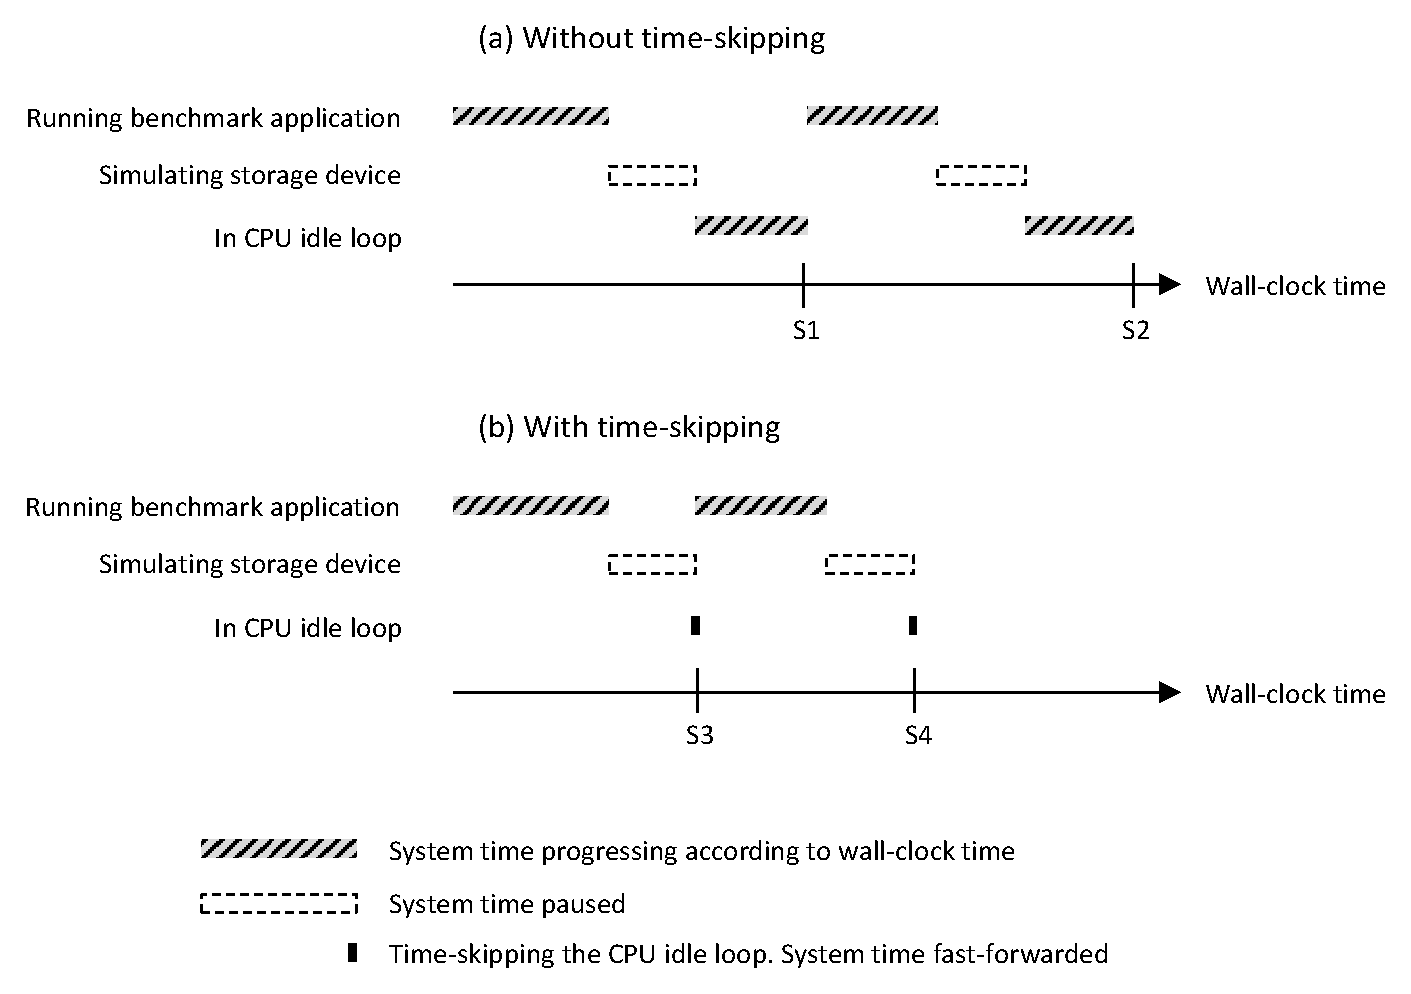
\includegraphics[width=1\textwidth]{figures/ch3-time-skipping.pdf}
	\caption{\label{fig:ch3-time-skipping}Example operation of CPU idle loop time-skipping.}
\end{figure}

An example operation of the CPU idle loop time-skipping feature is illustrated in Figure~\ref{fig:ch3-time-skipping}. This example illustrates a benchmark application submitting two I/O requests to the simulated storage device. The state of the OS is paused as soon as the I/O request is received by the simulated storage device. The work of simulating the I/O response is done while the OS is in the paused state (i.e., while the system time is paused). After the servicing time for the I/O response is determined, the OS will enter the idle mode to wait for the corresponding servicing time to pass by before it will receive the I/O response from the simulated storage device. With the CPU idle loop time-skipping feature, the actual waiting time in the CPU idle loop can be skipped. The OS state at S1 will be the same as the OS state at S3, and the OS state at S2 will be the same as the OS state at S4.

%Discuss the possible problem of "driver timeout".

When fast-forwarding the system time of the OS, special attention needs to be paid to device drivers that interact with real-world device entities. Some device drivers will have timeout mechanisms for detecting device errors. To maintain proper operation, theses timeout values will need to be adjusted accordingly taking into account the speedup ratio of the system time.